\documentclass[11pt,a4paper]{article}
\usepackage[T1]{fontenc}
\usepackage[utf8]{inputenc}
\usepackage[bahasa]{babel}
\usepackage{amsmath,amssymb}
\usepackage{booktabs}
\usepackage{graphicx}
\usepackage{siunitx}
\usepackage{geometry}
\usepackage{caption}
\geometry{margin=2.5cm}

\title{\textbf{Economic Dispatch 5 Pembangkit \\ dengan Metode \emph{Lambda-Iteration}}}
\author{Hero Yudo Martono \\ NRP. 1026900012 \\ S3 Sistem Siber Fisik --- PENS}
\date{\today}

\begin{document}

%============================= HALAMAN JUDUL =============================
\begin{titlepage}
\centering

% Logo PENS: letakkan berkas bernama logo-pens.png di folder yang sama.
% Jika logo belum tersedia, blok ini otomatis dilewati.
\IfFileExists{logo-pens.png}{%
  \includegraphics[height=3cm]{logo-pens.png}\par\vspace{1cm}%
}{%
  \vspace*{1cm}%
}

{\scshape\large Tugas Mata Kuliah Eval CPS\par}
\vspace{0.5cm}
{\scshape Economic Dispatch\par}
\vspace{2cm}

{\huge\bfseries Economic Dispatch 5 Pembangkit\par}
\vspace{0.4cm}
{\LARGE\bfseries dengan Metode \emph{Lambda-Iteration}\par}
\vspace{3cm}

{\large\bfseries Disusun oleh:\par}
\vspace{0.4cm}
{\large Hero Yudo Martono\par}
{\large NRP. 1026900012\par}
\vspace{2cm}

{\large Program Studi S3 Sistem Siber Fisik\par}
{\large Politeknik Elektronika Negeri Surabaya (PENS)\par}
\vspace{1cm}
{\large \today\par}

\vfill
\end{titlepage}
%========================================================================

\maketitle

\section{Deskripsi Masalah}
\emph{Economic dispatch} (ED) menentukan daya keluaran setiap generator agar
\textbf{total biaya pembangkitan minimum} sambil memenuhi beban sistem dan batas
operasi tiap unit. Fungsi biaya tiap generator berbentuk kuadratik:
\begin{equation}
C_i(P_i) = a_i P_i^2 + b_i P_i + c_i \quad (\si{\$/jam}).
\end{equation}
Masalah optimasi:
\begin{equation}
\min \; \sum_{i=1}^{5} C_i(P_i)
\quad\text{dengan kendala}\quad
\sum_{i=1}^{5} P_i = P_D, \qquad P_i^{\min} \le P_i \le P_i^{\max}.
\end{equation}

\begin{table}[h]
\centering
\caption{Data lima pembangkit (biaya kuadratik dan batas daya).}
\begin{tabular}{lccccc}
\toprule
Gen & $P^{\min}$ (MW) & $P^{\max}$ (MW) & $a$ & $b$ & $c$ \\
\midrule
G1 & 0 & 300 & 0,002 & 10 & 100 \\
G2 & 0 & 250 & 0,003 & 8  & 120 \\
G3 & 0 & 200 & 0,004 & 6  & 150 \\
G4 & 0 & 150 & 0,005 & 5  & 180 \\
G5 & 0 & 100 & 0,006 & 4  & 200 \\
\bottomrule
\end{tabular}
\end{table}

Ketiga koefisien biaya pada Tabel~1 memiliki makna fisik sebagai berikut:
\begin{itemize}
  \item $c_i$ --- \textbf{biaya tetap} (\emph{fixed/no-load cost}), bersatuan \si{\$/jam}.
  Biaya yang tetap muncul selama unit menyala meski keluaran daya kecil (menjaga
  boiler/turbin tetap siap, biaya operasional dasar); tidak bergantung pada $P_i$.
  \item $b_i$ --- \textbf{koefisien biaya linear}, bersatuan \si{\$/MWh}. Mewakili
  komponen biaya yang sebanding dengan daya (mendekati biaya bahan bakar per satuan
  energi). Nilai $b$ yang lebih kecil berarti unit lebih murah di margin, sehingga
  diprioritaskan lebih dulu.
  \item $a_i$ --- \textbf{koefisien biaya kuadratik}, bersatuan \si{\$/MWh\squared}.
  Menangkap efek \emph{efisiensi menurun}: makin tinggi daya, biaya tambahan per MW
  makin naik. Suku ini membuat kurva biaya \emph{konveks} sehingga \emph{economic
  dispatch} memiliki solusi optimum tunggal.
\end{itemize}

Konsekuensinya, biaya marjinal (\emph{incremental cost}) tiap unit adalah
$dC_i/dP_i = 2a_i P_i + b_i$: $b_i$ adalah biaya marjinal saat daya nol dan $2a_i P_i$
adalah kenaikannya seiring bertambahnya daya --- besaran inilah yang disamakan
menjadi $\lambda$ pada metode \emph{lambda-iteration}.

Beban yang dioptimalkan: $P_D = \SI{650}{MW}$ dan $P_D = \SI{740}{MW}$.
Keduanya layak karena $\sum P^{\min}=0 \le P_D \le \sum P^{\max}=\SI{1000}{MW}$.

\section{Pemilihan Metode}
Fungsi biaya berbentuk kuadratik dengan kendala linear, sehingga masalah ini
\textbf{konveks} dan memiliki solusi optimal \emph{eksak dan tunggal}. Untuk kasus
seperti ini, metode \textbf{\emph{lambda-iteration}} adalah pilihan paling tepat
karena: (i) menemukan optimum global secara pasti (bukan hampiran stokastik);
(ii) bersifat iteratif sehingga sesuai dengan ketentuan \emph{iterasi maksimum $=50$}
dan langsung menghasilkan \textbf{kurva biaya terhadap iterasi} yang diminta;
(iii) merupakan metode baku \emph{economic dispatch} pada literatur sistem tenaga
(Wood \& Wollenberg); dan (iv) hasilnya dapat diverifikasi manual melalui syarat
kesamaan \emph{incremental cost}. Metode metaheuristik (PSO/GA) tidak diperlukan
karena masalah konveks ini tidak memiliki banyak optimum lokal; QP satu-langkah
tidak menghasilkan jejak per-iterasi yang diminta tugas.

\section{Metode Optimasi: \emph{Lambda-Iteration}}
Pada titik optimum (tanpa rugi saluran), \emph{incremental cost} setiap unit yang
tidak berada di batas bernilai sama, yaitu sebesar $\lambda$:
\begin{equation}
\frac{dC_i}{dP_i} = 2a_i P_i + b_i = \lambda
\;\Longrightarrow\;
P_i(\lambda) = \operatorname{clip}\!\left(\frac{\lambda - b_i}{2a_i},\; P_i^{\min},\; P_i^{\max}\right).
\end{equation}
Secara satuan, $\lambda$ adalah \emph{incremental cost}, yaitu turunan biaya ($\si{\$/jam}$)
terhadap daya ($\si{MW}$), sehingga bersatuan $\si{\$/MWh}$; ia menyatakan biaya marjinal
sistem untuk memasok satu MW tambahan.

Nilai $\lambda$ dicari secara iteratif (\textbf{bisection}) agar keseimbangan daya
$\sum_i P_i(\lambda) = P_D$ terpenuhi:
\begin{enumerate}
  \item Tetapkan selang awal $[\lambda_{\text{lo}}, \lambda_{\text{hi}}]$ dari rentang
  \emph{incremental cost} semua unit.
  \item Ambil $\lambda = \tfrac{1}{2}(\lambda_{\text{lo}}+\lambda_{\text{hi}})$,
  hitung $P_i(\lambda)$ dan $\sum_i P_i$.
  \item Jika $\sum_i P_i > P_D$ turunkan $\lambda_{\text{hi}}\!=\!\lambda$; jika
  $\sum_i P_i < P_D$ naikkan $\lambda_{\text{lo}}\!=\!\lambda$.
  \item Ulangi sampai \textbf{iterasi maksimum $=50$}. Biaya total dan daya tiap unit
  dicatat pada setiap iterasi untuk grafik konvergensi.
\end{enumerate}

\section{Hasil Optimasi}

\subsection{Beban $P_D = \SI{650}{MW}$}
Nilai konvergen: $\lambda = \SI{9,20}{\$/MWh}$, total biaya
$\boxed{\SI{5152,50}{\$/jam}}$.
\begin{table}[h]
\centering
\caption{Dispatch optimal pada beban 650 MW.}
\begin{tabular}{lcccc}
\toprule
Gen & $P_i$ (MW) & $IC = 2a_iP_i+b_i$ & $C_i$ (\$/jam) & Status \\
\midrule
G1 & 0{,}00   & 10{,}00 & 100{,}00  & di $P^{\min}$ \\
G2 & 200{,}00 & 9{,}20  & 1840{,}00 & bebas ($IC=\lambda$) \\
G3 & 200{,}00 & 7{,}60  & 1510{,}00 & di $P^{\max}$ \\
G4 & 150{,}00 & 6{,}50  & 1042{,}50 & di $P^{\max}$ \\
G5 & 100{,}00 & 5{,}20  & 660{,}00  & di $P^{\max}$ \\
\midrule
\textbf{Total} & \textbf{650{,}00} & & \textbf{5152{,}50} & \\
\bottomrule
\end{tabular}
\end{table}

\subsection{Beban $P_D = \SI{740}{MW}$}
Nilai konvergen: $\lambda = \SI{10,16}{\$/MWh}$, total biaya
$\boxed{\SI{6023,20}{\$/jam}}$.
\begin{table}[h]
\centering
\caption{Dispatch optimal pada beban 740 MW.}
\begin{tabular}{lcccc}
\toprule
Gen & $P_i$ (MW) & $IC = 2a_iP_i+b_i$ & $C_i$ (\$/jam) & Status \\
\midrule
G1 & 40{,}00  & 10{,}16 & 503{,}20  & bebas ($IC=\lambda$) \\
G2 & 250{,}00 & 9{,}50  & 2307{,}50 & di $P^{\max}$ \\
G3 & 200{,}00 & 7{,}60  & 1510{,}00 & di $P^{\max}$ \\
G4 & 150{,}00 & 6{,}50  & 1042{,}50 & di $P^{\max}$ \\
G5 & 100{,}00 & 5{,}20  & 660{,}00  & di $P^{\max}$ \\
\midrule
\textbf{Total} & \textbf{740{,}00} & & \textbf{6023{,}20} & \\
\bottomrule
\end{tabular}
\end{table}

\section{Grafik Konvergensi}
Grafik berikut menampilkan \textbf{total biaya pembangkitan terhadap iterasi}
(sumbu-$x$ = iterasi, sumbu-$y$ = biaya) untuk kedua beban. Metode
\emph{lambda-iteration} meredam osilasi awal dan konvergen stabil dalam kurang dari
15 iterasi, lalu tetap konstan hingga iterasi ke-50.

\begin{figure}[h]
\centering
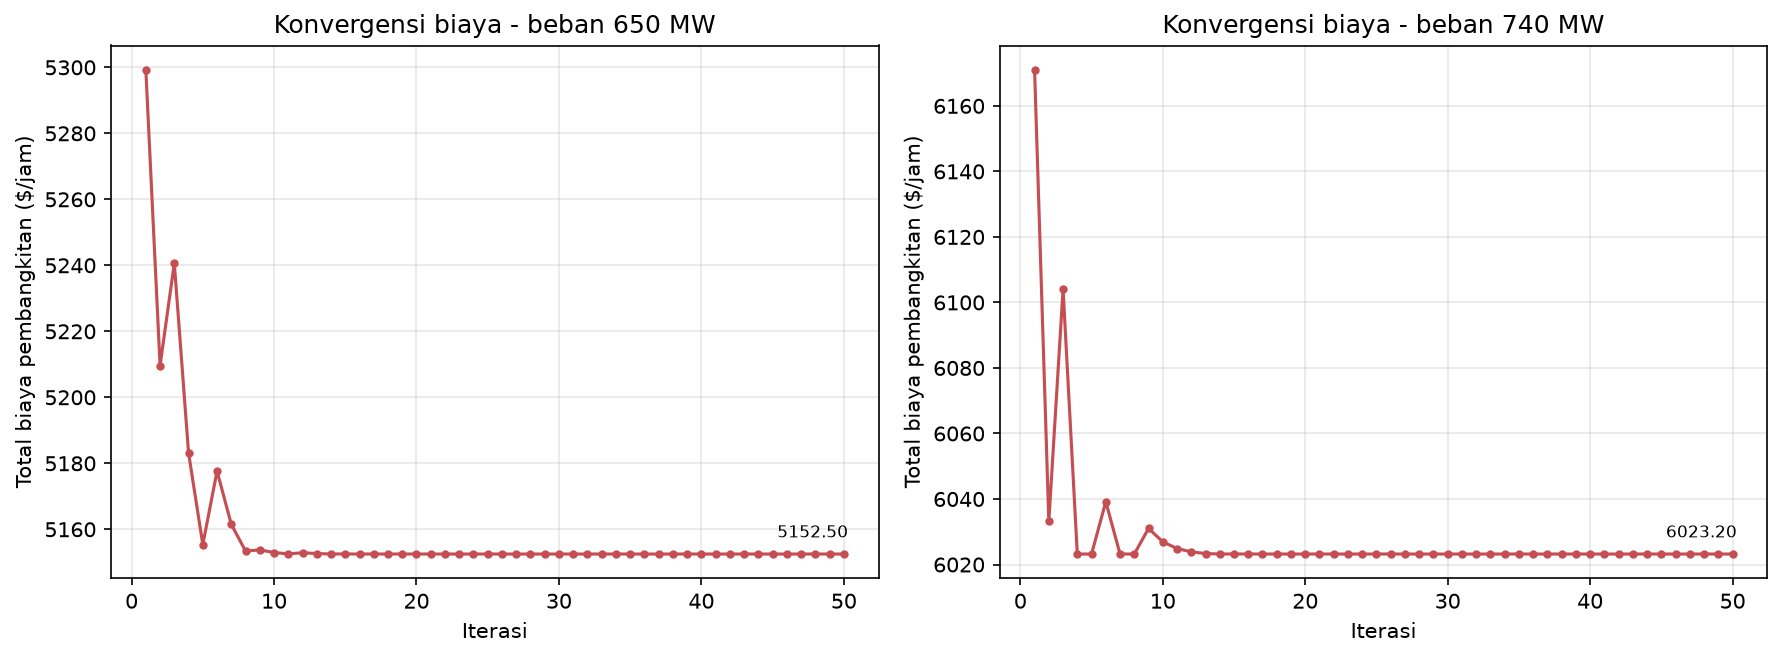
\includegraphics[width=\linewidth]{ed_cost_convergence.png}
\caption{Konvergensi total biaya pembangkitan vs iterasi (kiri: 650 MW, kanan: 740 MW).}
\end{figure}

\begin{figure}[h]
\centering
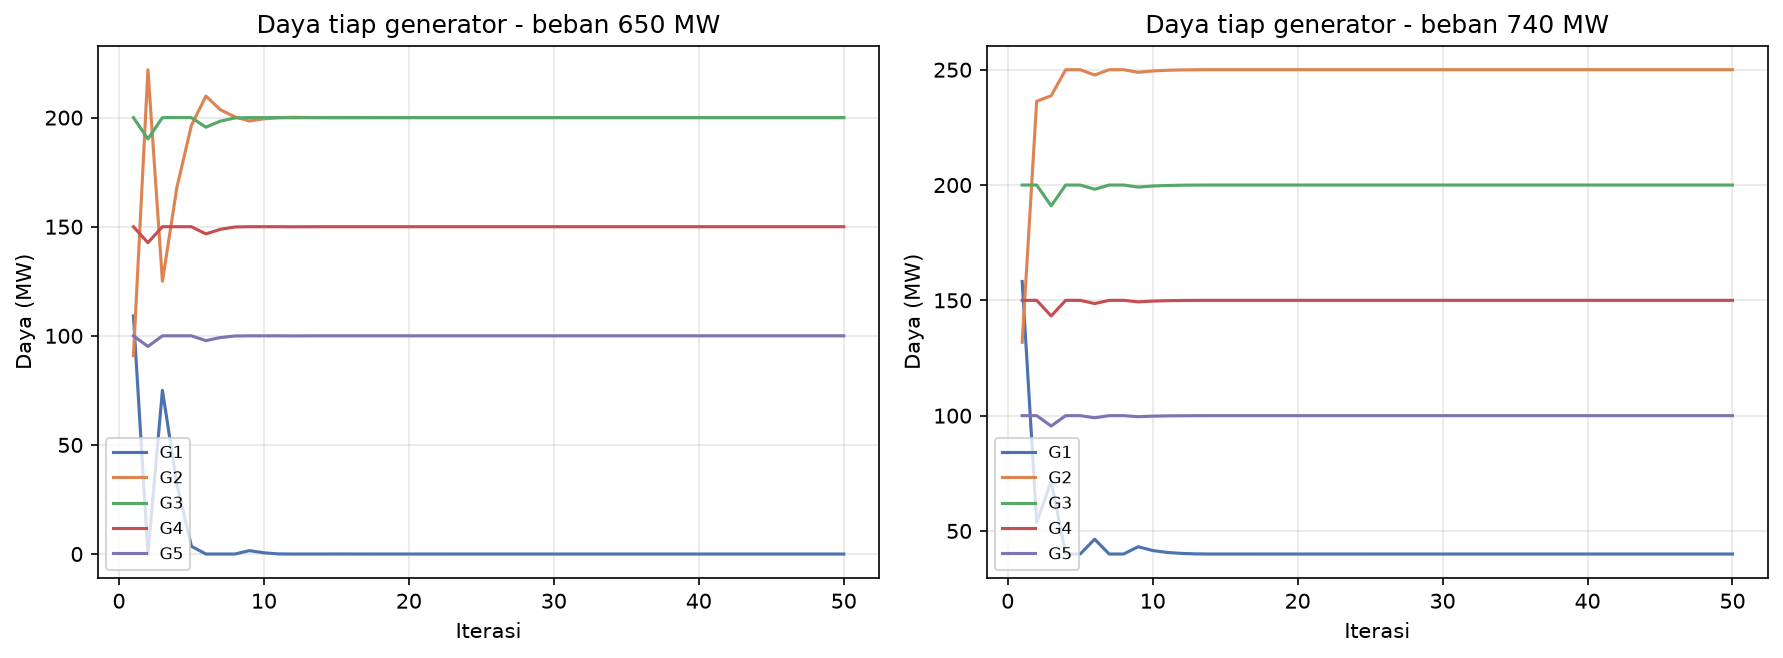
\includegraphics[width=\linewidth]{ed_power_convergence.png}
\caption{Perubahan daya tiap generator sepanjang iterasi (kiri: 650 MW, kanan: 740 MW).}
\end{figure}

\section{Analisis}
\begin{itemize}
  \item \textbf{Urutan prioritas pembangkitan} mengikuti koefisien biaya marjinal.
  Karena $b$ menurun dari G1 ($b=10$) ke G5 ($b=4$), unit termurah di margin (G5, G4,
  G3) dibebani hingga $P^{\max}$ lebih dulu, sedangkan unit termahal (G1) baru dihidupkan
  ketika beban cukup besar.
  \item Pada \textbf{650 MW}, G1 mati ($P=0$); hanya G2 yang menjadi unit \emph{bebas}
  sehingga \emph{incremental cost}-nya tepat sama dengan $\lambda=9{,}20$. Unit lain yang
  berada di batas boleh memiliki $IC \ne \lambda$ --- ini konsisten dengan syarat
  Karush--Kuhn--Tucker ketika kendala batas aktif.
  \item Pada \textbf{740 MW}, beban tambahan 90 MW diserap dengan menaikkan G2 ke
  $P^{\max}=250$ dan menghidupkan G1 sebesar 40 MW ($IC_{G1}=\lambda=10{,}16$).
  \item \textbf{Kenaikan biaya} dari 650 MW ke 740 MW sebesar
  $6023{,}20-5152{,}50 = \SI{870,70}{\$/jam}$ untuk tambahan 90 MW
  ($\approx \SI{9,67}{\$/MWh}$ rata-rata), sejalan dengan rentang $\lambda$ yang naik dari
  9,20 menjadi 10,16 \$/MWh.
  \item \textbf{Konvergensi:} \emph{bisection} pada $\lambda$ sendiri konvergen monoton
  (selang $[\lambda_{\text{lo}},\lambda_{\text{hi}}]$ selalu menyempit). Lonjakan kecil pada
  kurva biaya iterasi awal (mis. beban 740 MW di iterasi ke-6--9) adalah \emph{artefak
  pelaporan}: biaya dihitung pada dispatch yang telah diproyeksikan agar $\sum P_i=P_D$
  meskipun $\lambda$ belum presisi --- \textbf{bukan} ketidakstabilan metode. Setelah
  $\lambda$ konvergen (<15 iterasi), biaya stabil dan pada iterasi ke-50 identik dengan
  solusi optimal.
\end{itemize}

\section{Verifikasi Silang (Validasi Hasil)}
Untuk memastikan solusi \emph{lambda-iteration} benar-benar optimum global (bukan
terjebak di titik suboptimal), hasil dibandingkan dengan \emph{solver} optimasi
independen \textbf{SLSQP} (\emph{Sequential Least-Squares Quadratic Programming},
pustaka \texttt{scipy.optimize}) pada problem yang sama. Kedua metode memberikan hasil
\textbf{identik}:
\begin{center}
\begin{tabular}{lcc}
\toprule
 & Beban 650 MW & Beban 740 MW \\
\midrule
Lambda-iteration (\$/jam) & 5152{,}50 & 6023{,}20 \\
SLSQP (\$/jam)            & 5152{,}50 & 6023{,}20 \\
Selisih                   & 0{,}00 & 0{,}00 \\
\bottomrule
\end{tabular}
\end{center}
Kesamaan ini mengonfirmasi bahwa dispatch yang diperoleh adalah \textbf{optimum global}
untuk kedua beban.

\section{Kesimpulan}
Dengan metode \emph{lambda-iteration} (maks 50 iterasi), diperoleh dispatch ekonomis:
\begin{center}
\begin{tabular}{lcc}
\toprule
 & Beban 650 MW & Beban 740 MW \\
\midrule
$\lambda$ (\$/MWh) & 9{,}20 & 10{,}16 \\
Total biaya (\$/jam) & \textbf{5152{,}50} & \textbf{6023{,}20} \\
$(P_{G1},\dots,P_{G5})$ (MW) & $(0,200,200,150,100)$ & $(40,250,200,150,100)$ \\
\bottomrule
\end{tabular}
\end{center}

Perhitungan dan grafik dihasilkan oleh \texttt{economic\_dispatch.ipynb} (Python);
seluruh angka berasal dari eksekusi nyata, dapat direproduksi.

\end{document}
